% SETUP
\documentclass{article}
\usepackage{geometry}
\usepackage{fancyhdr}
\usepackage{titlesec}
\usepackage{tabularx}
\usepackage[none]{hyphenat}
\usepackage{multicol}
\usepackage{hhline}
\usepackage{caption}
\usepackage{graphicx}
\usepackage{biblatex}
\addbibresource{references.bib}
\geometry{
	a4paper, 
	total={170mm,257mm}, 
	left=25mm, 
	right=25mm,
	top=30mm, 
	bottom=30mm}

% FIGURES IN MULTICOLS
\newenvironment{Figure}
  {\par\medskip\noindent\minipage{\linewidth}}
  {\endminipage\par\medskip}

% SECTION TITLE FORMAT
\titleformat{\section}
  {\normalfont\bfseries}{\thesection}{1em}{}[{\titlerule[0.3pt]}]

% HEADER & FOOTER
\pagestyle{fancy}
\renewcommand{\headrulewidth}{0pt}
\chead{\large Assignment Report: Machine Learning Applications for Computer Graphics}
\lhead{}
\rhead{}
\cfoot{}

\begin{document}

% CONTACT
\begin{table}[!h]
\center
\begin{tabular}{|l|l|l|}
\hline
\textbf{Name}             & \textbf{Student ID} & \textbf{E-Mail}            \\ \hhline{|=|=|=|}
Li Nguyen        & 934644485  & li.nguyen@tum.de  \\ \hline
Alexander Koenig & 918254061  & awc.koenig@tum.de \\ \hline
\end{tabular}
\end{table}

\begin{figure}[h!]
	\centering 
	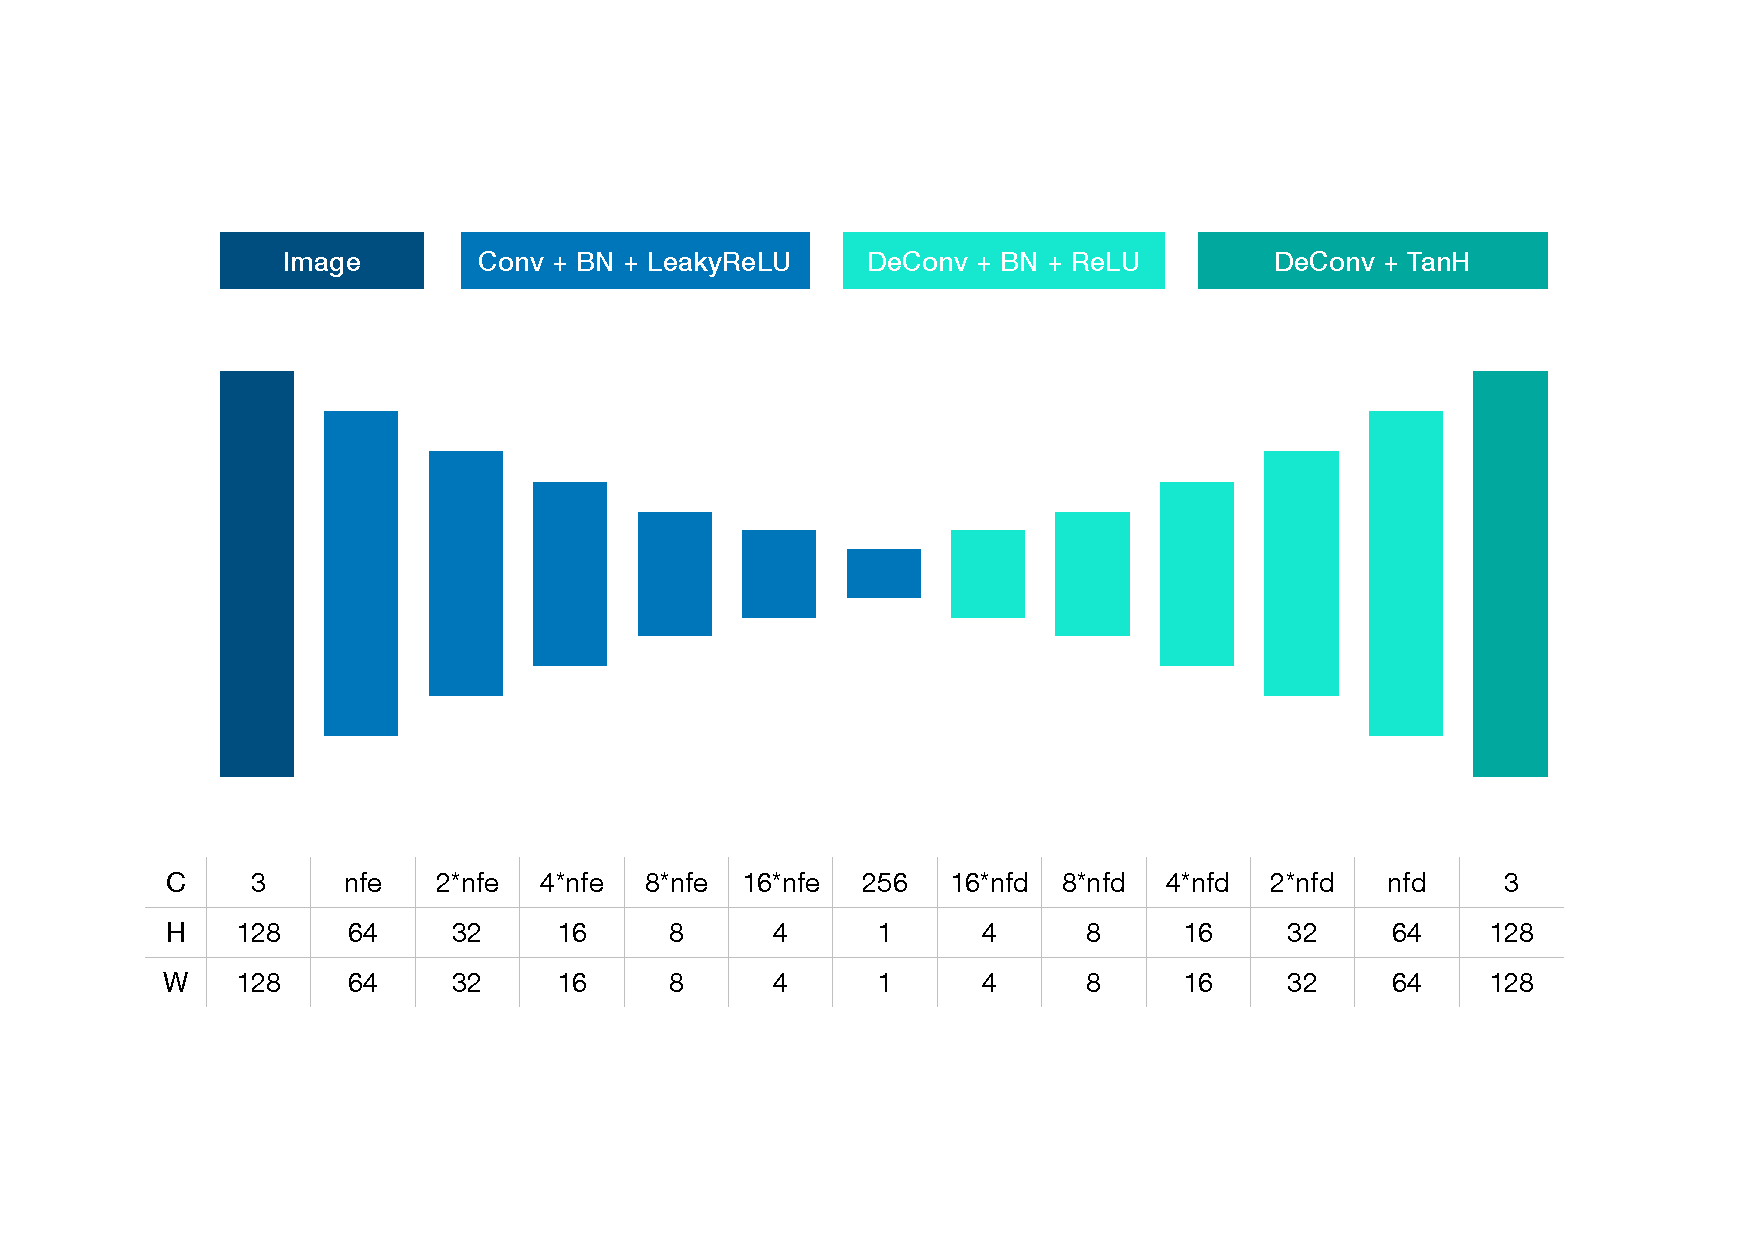
\includegraphics[width=0.9\linewidth]{figures/ae_1}
	\caption{Architecture and output shapes for autoencoder model 1}
	\label{fig:model1}
\end{figure}

\begin{figure}[t!]
	\centering 
	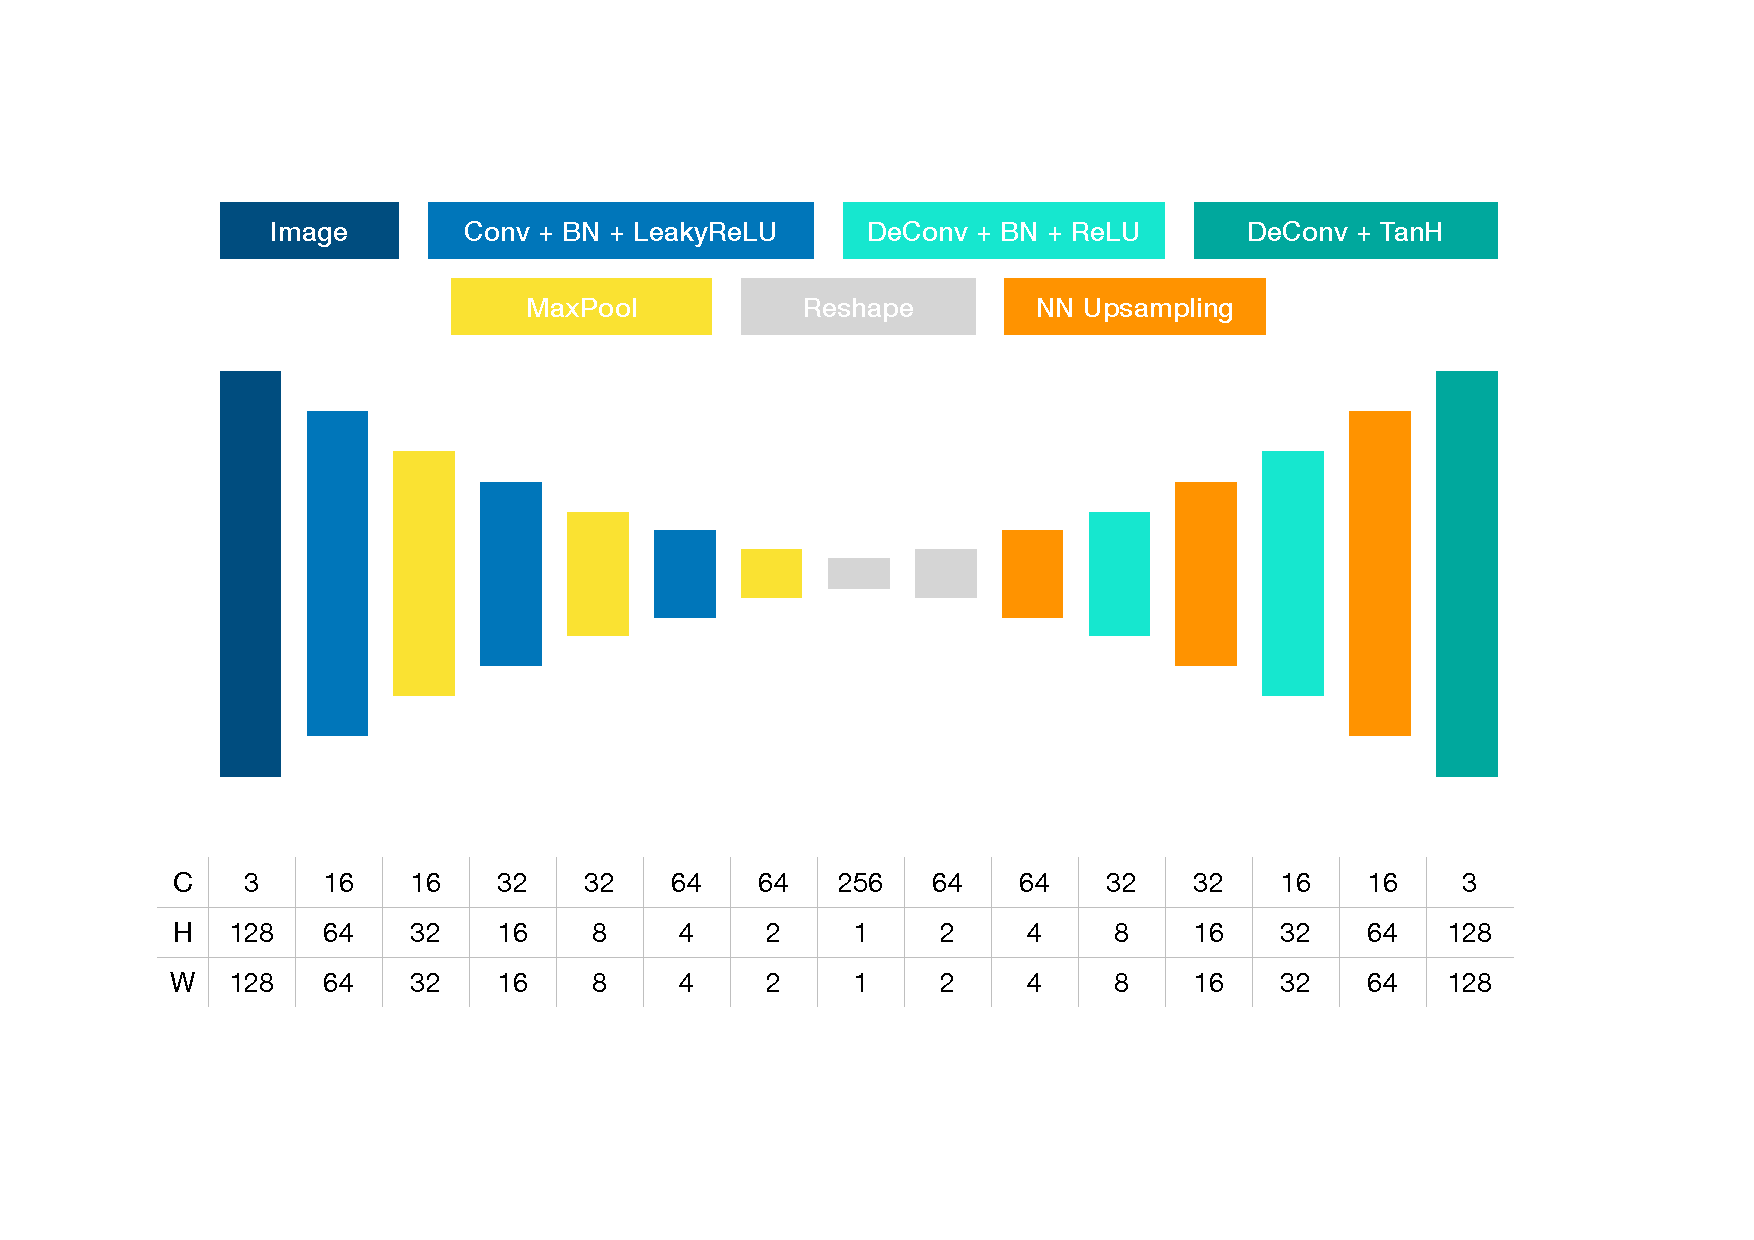
\includegraphics[width=0.9\linewidth]{figures/ae_2}
	\caption{Architecture and output shapes for autoencoder model 2}
	\label{fig:model2}
\end{figure}

\begin{figure}[t]
	\centering 
	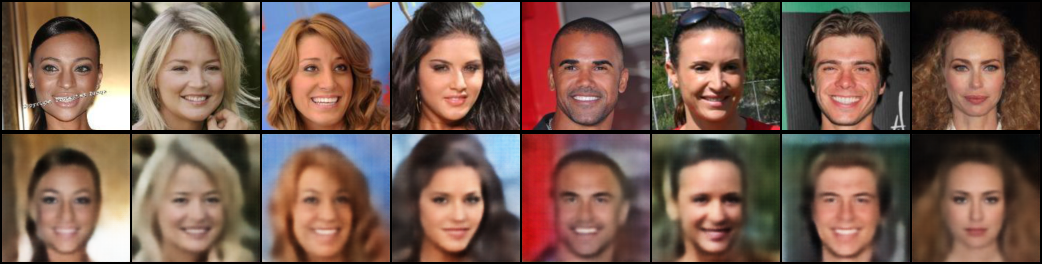
\includegraphics[width=0.95\linewidth]{figures/imgs_model_1}
	
	\vspace{0.5cm}
	
	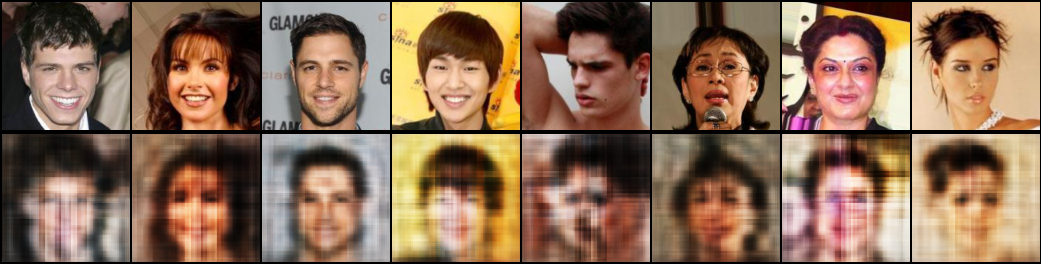
\includegraphics[width=0.95\linewidth]{figures/imgs_model_2}
	\caption{Test images produced by model 1 (top) and model 2 (bottom) with inputs}
	\label{fig:images}
\end{figure}

\begin{multicols}{2}

\section{Introduction}

Autoencoders are a neural network paradigm that aim to produce a meaningful lower dimensional representation of some input data in an unsupervised manner. Autoencoders employ an encoder-decoder structure. The encoder $E(x)$ produces the low dimensional representation $z$ of the input data $x$ in a so called bottleneck. The decoder $D(z)$ then aims to reconstruct the original input from the compact information contained in the bottleneck. The training goal is to minimize the reconstruction loss (i.e. the output of the decoder should be as close as possible to the original input). Applications of autoencoders include dimensionality reduction, anomaly detection and feature extraction. 

In this report we describe a deep convolutional autoencoder that compresses images of celebrities of size (3 $\times$ 128 $\times$ 128 = 49152 entries) in a bottleneck of size (256 $\times$ 1 $\times$ 1). This corresponds to a compression of 95.31\%.

\section{Architectures}
\textbf{Model 1}: Figure \ref{fig:model1} shows the architecture of our first deep convolutional autoencoder. The table in figure \ref{fig:model1} shows its output dimensions. There are two variables in the table: $n_{fe}$ and $n_{fd}$. They describe the number of feature maps in the first and last layers of the encoder and decoder, respectively. These parameters are hyper-parameters and are assessed in a grid search process. 

In the encoder, the height and width of the original image (128 $\times$ 128) is downscaled by a factor of 2 at each convolutional layer. To achieve this we use a kernel size of 4 $\times$ 4, stride 2 and padding 1 for the convolutions, except in the layer before the bottleneck. In this layer we use 256 filters with a kernel size of 4 $\times$ 4, stride 1 and padding 0 to reach the desired shape of 256 $\times$ 1 $\times$ 1 in the bottleneck. 

In the decoder, the de-convolutional layers upsample the height and width of the layers by a factor of 2 until the output dimensions are reached. In every layer except the last one the (de)-convolutional layer is followed by a BatchNorm operation and a LeakyReLU activation for the encoder and a ReLU activation for the decoder. The last convolutional layer in the decoder is followed by a $tanh()$ operation to produce bounded RGB values in the output image.

\textbf{Model 2}: In a second model we try to propose a more lightweight architecture with fewer parameters. We swap every other layer of the first model with max pooling operations in the encoder and nearest neighbour upsampling in the decoder (see Figure \ref{fig:model2}). For the max pooling operations we use a kernel size of 2 $\times$ 2 with stride 2 and padding 0. Hence, after each max pooling layer the height and width of the images is reduced by a factor of 2. The output shape of the last max pooling operation in the encoder is (64 $\times$ 2 $\times$ 2). We flatten this output to reach the desired shape of (256 $\times$ 1 $\times$ 1) in the bottleneck. In the first layer of the decoder we reshape again to reach dimensions of (64 $\times$ 2 $\times$ 2). In the decoder we use nearest neighbour upsampling to scale the height and width of the feature maps up by a factor of 2.

\section{Optimization}
Both models use the mean squared error (MSE) as their loss function. Let $x_i$ be one of $n$ images, then the output of the autoencoder after encoding and decoding is $\hat{x}_i = D(E(x_i))$. Due to the high compression some information from the original image is lost. We aim to minimize the following reconstruction error.
\begin{equation}
	MSE = \frac{1}{n} \sum_{i=1}^n (x_i - \hat{x}_i)^2
\end{equation}

We use the Adam optimizer with learning rate 0.0002, $\beta_1 = 0.9$ and $\beta_2 = 0.999$ if not stated otherwise. 

\section{Dataset}

We use the CelebA dataset to train the autoencoders. We use the same train, validation and test split as in the original paper \cite{liu2015faceattributes}: 162770 training images (80\%), 19867 validation images (10\%) and 19962 test images (10\%). The dataset holds 202599 images in total. All images in this report are generated from the previously unseen test set.

\section{Results and Discussion}

\textbf{Experiment 1}: To compare the performance of both models we choose $n_{fe}=n_{fd}=16$ for model 1 such that both models have the same number of feature maps at the outermost layers. We run the experiments with a maximum of 8 training epochs. While the max pooling and upsampling layers in model 2 reduce the number of parameters of model 2 significantly and also increase training speed, its performance suffers dramatically. This is both evident from the losses and the visual quality of the images produced at test time. 

Figure \ref{fig:val} shows that the validation losses for model 2 are substantially higher than for model 1. This plot also suggests, that a larger batch size increases performance. Similarly, the training loss in figure \ref{fig:train} paints an equivalent picture. 

\begin{Figure}
	\centering 
	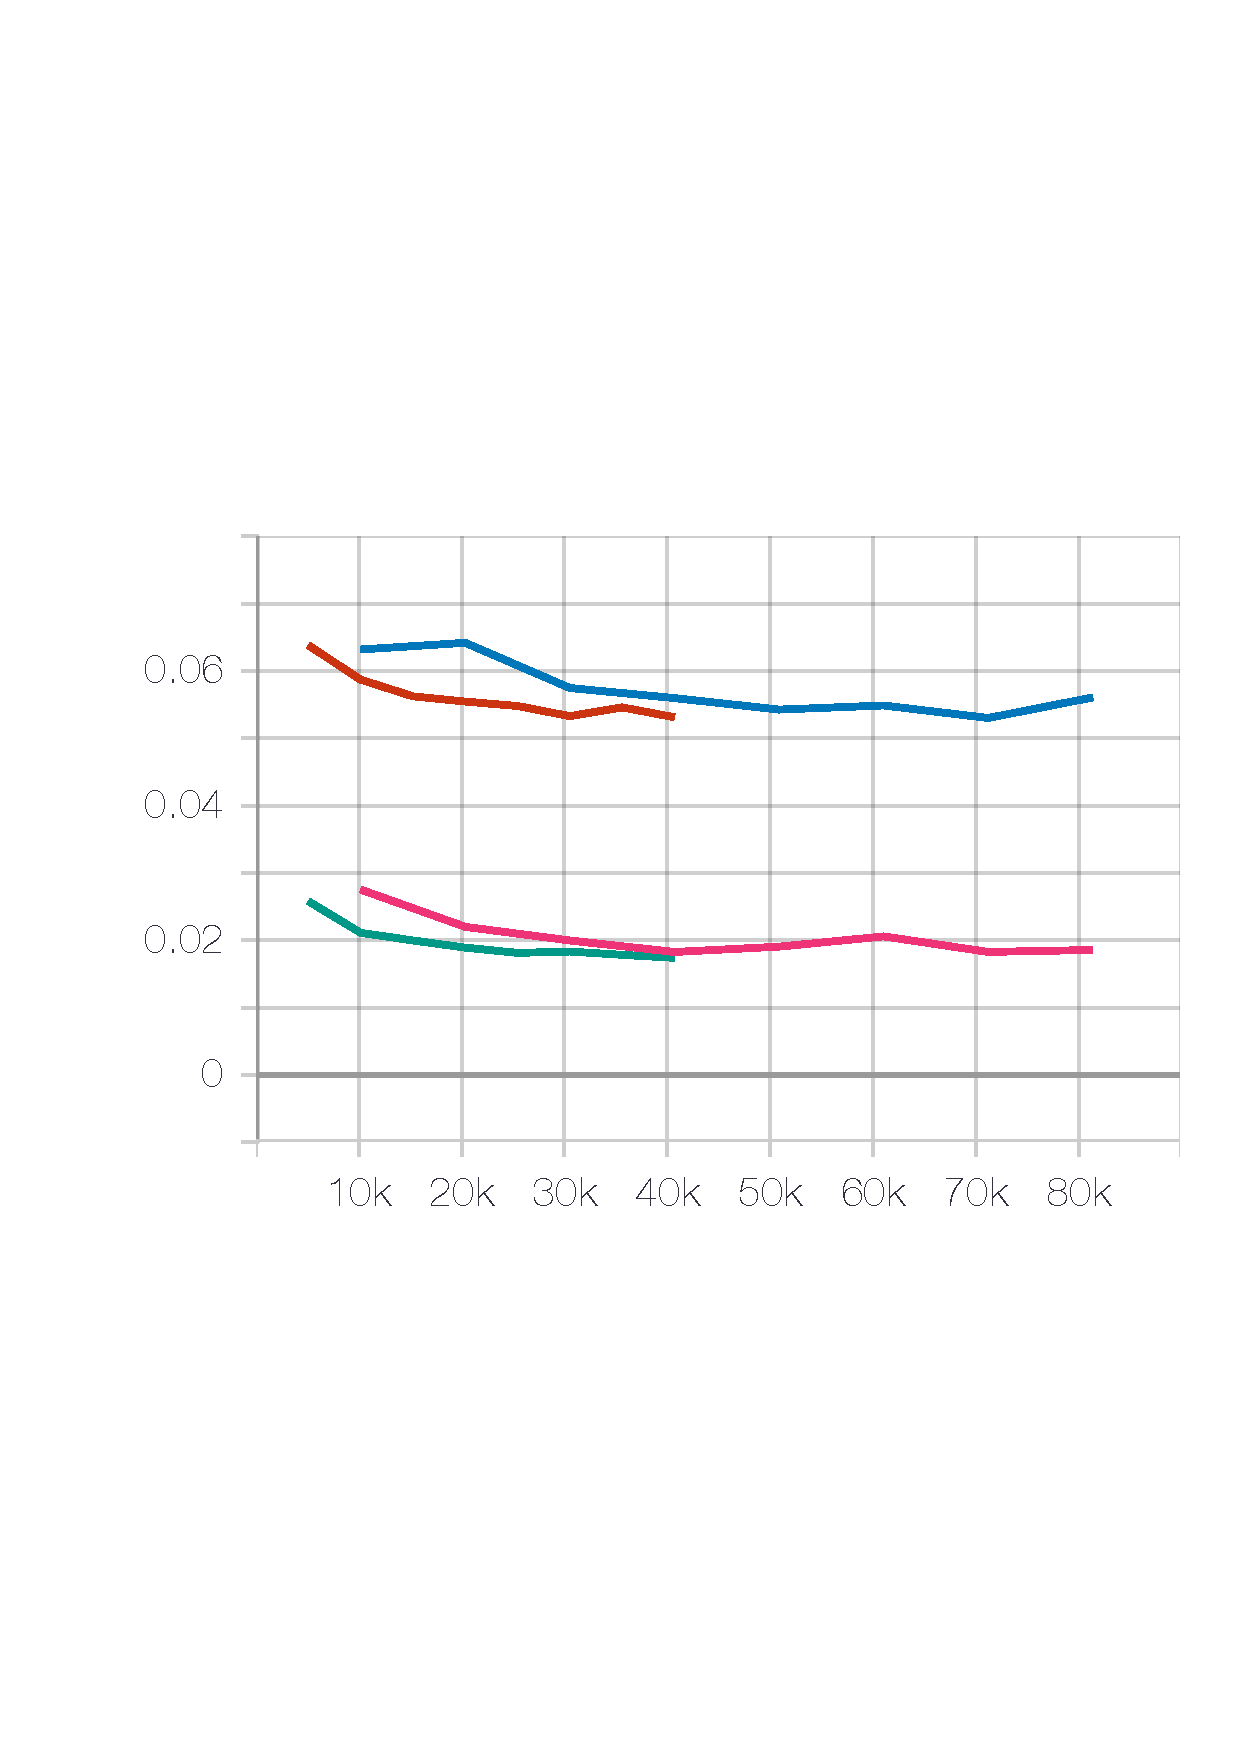
\includegraphics[width=\linewidth]{figures/val_1_2.pdf}
	\captionof{figure}{Validation losses for model 1  (\textit{pink}: batch size 16, \textit{green}: batch size 32) and model 2 (\textit{blue}: batch size 16, \textit{red}: batch size 32)}
	\label{fig:val}
\end{Figure}

Figure \ref{fig:images} shows a visual comparison between the images produced by model 1 and model 2 (both trained with batch size 32). From the loss plots as well as from the produced visual outputs it is clearly evident that model 1 performs better. The max pooling layers lead to an aggressive compression of the data in the encoder through which important information is lost in the encoding process. The decoder can not reconstruct a meaningful image from this representation. Further, the max pool operations in combination with the nearest neighbour upsampling seem to introduce rectangular patches into the output image. Most likely, this is due to the rectangular kernel of the nearest neighbour upsampling process. Regions of high detail and contrast such as facial landmarks (eyes, nose, mouth, etc.) seem to be especially prone to this distortion. The rectangular distortions seem to be less prominent in regions of low contrast such as the background.

\begin{Figure}
	\centering 
	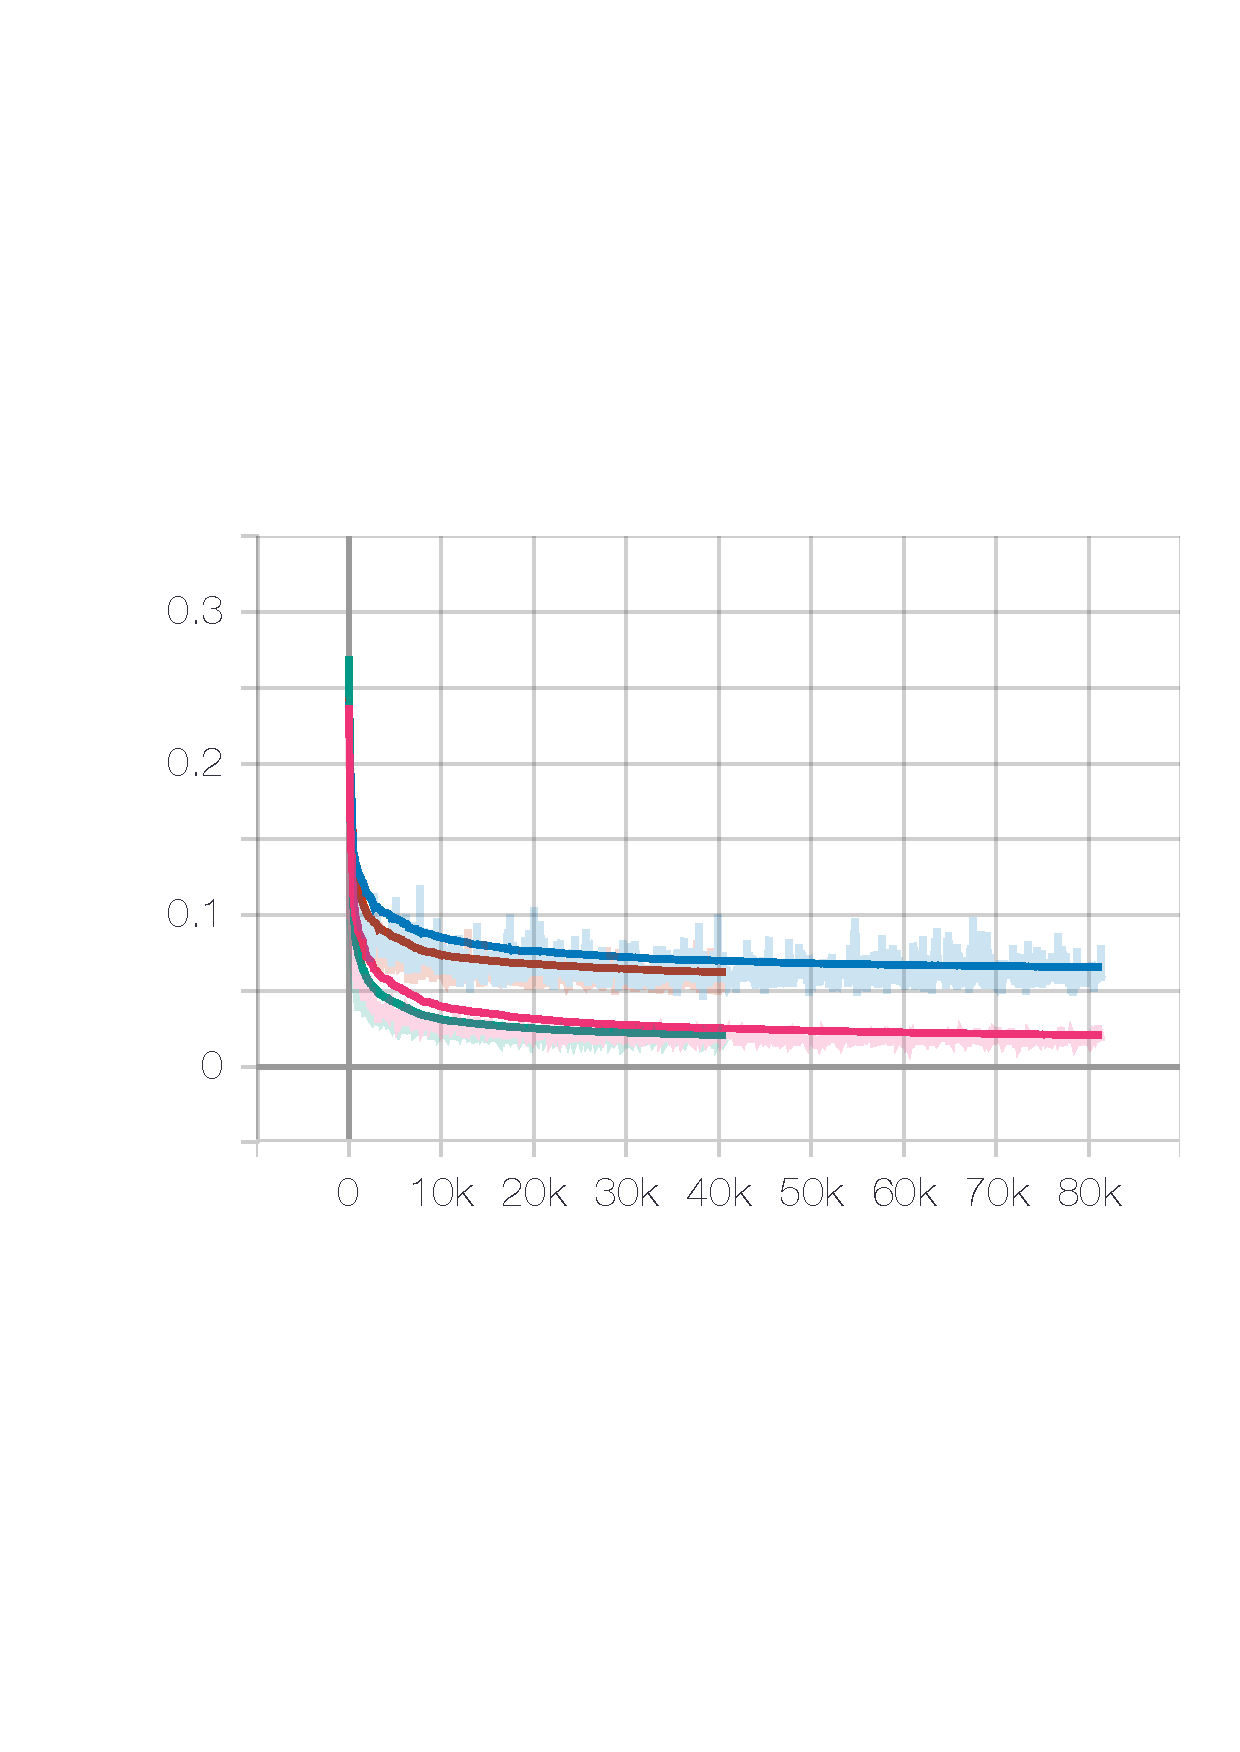
\includegraphics[width=\linewidth]{figures/train_1_2.pdf}
	\captionof{figure}{Training losses for model 1  (\textit{pink}: batch size 16, \textit{green}: batch size 32) and model 2 (\textit{blue}: batch size 16, \textit{red}: batch size 32)}
	\label{fig:train}
\end{Figure}

\textbf{Experiment 2}: Due to the poor results of model 2 we decided to run more tests on model 1. We tried different batch sizes and $n_{fe}$ and $n_{fd}$ combinations in a grid search process. We denote $n_{fe} = n_{fd} = n_{f}$ since we keep the number of feature maps in the encoder and decoder symmetric. There seems to be a positive correlation between the output quality and higher batch sizes as well as more feature maps. This is evident from figure \ref{fig:val_grid}. Like before all models were trained for a maximum number of 8 epochs.

\begin{Figure}
	\centering 
	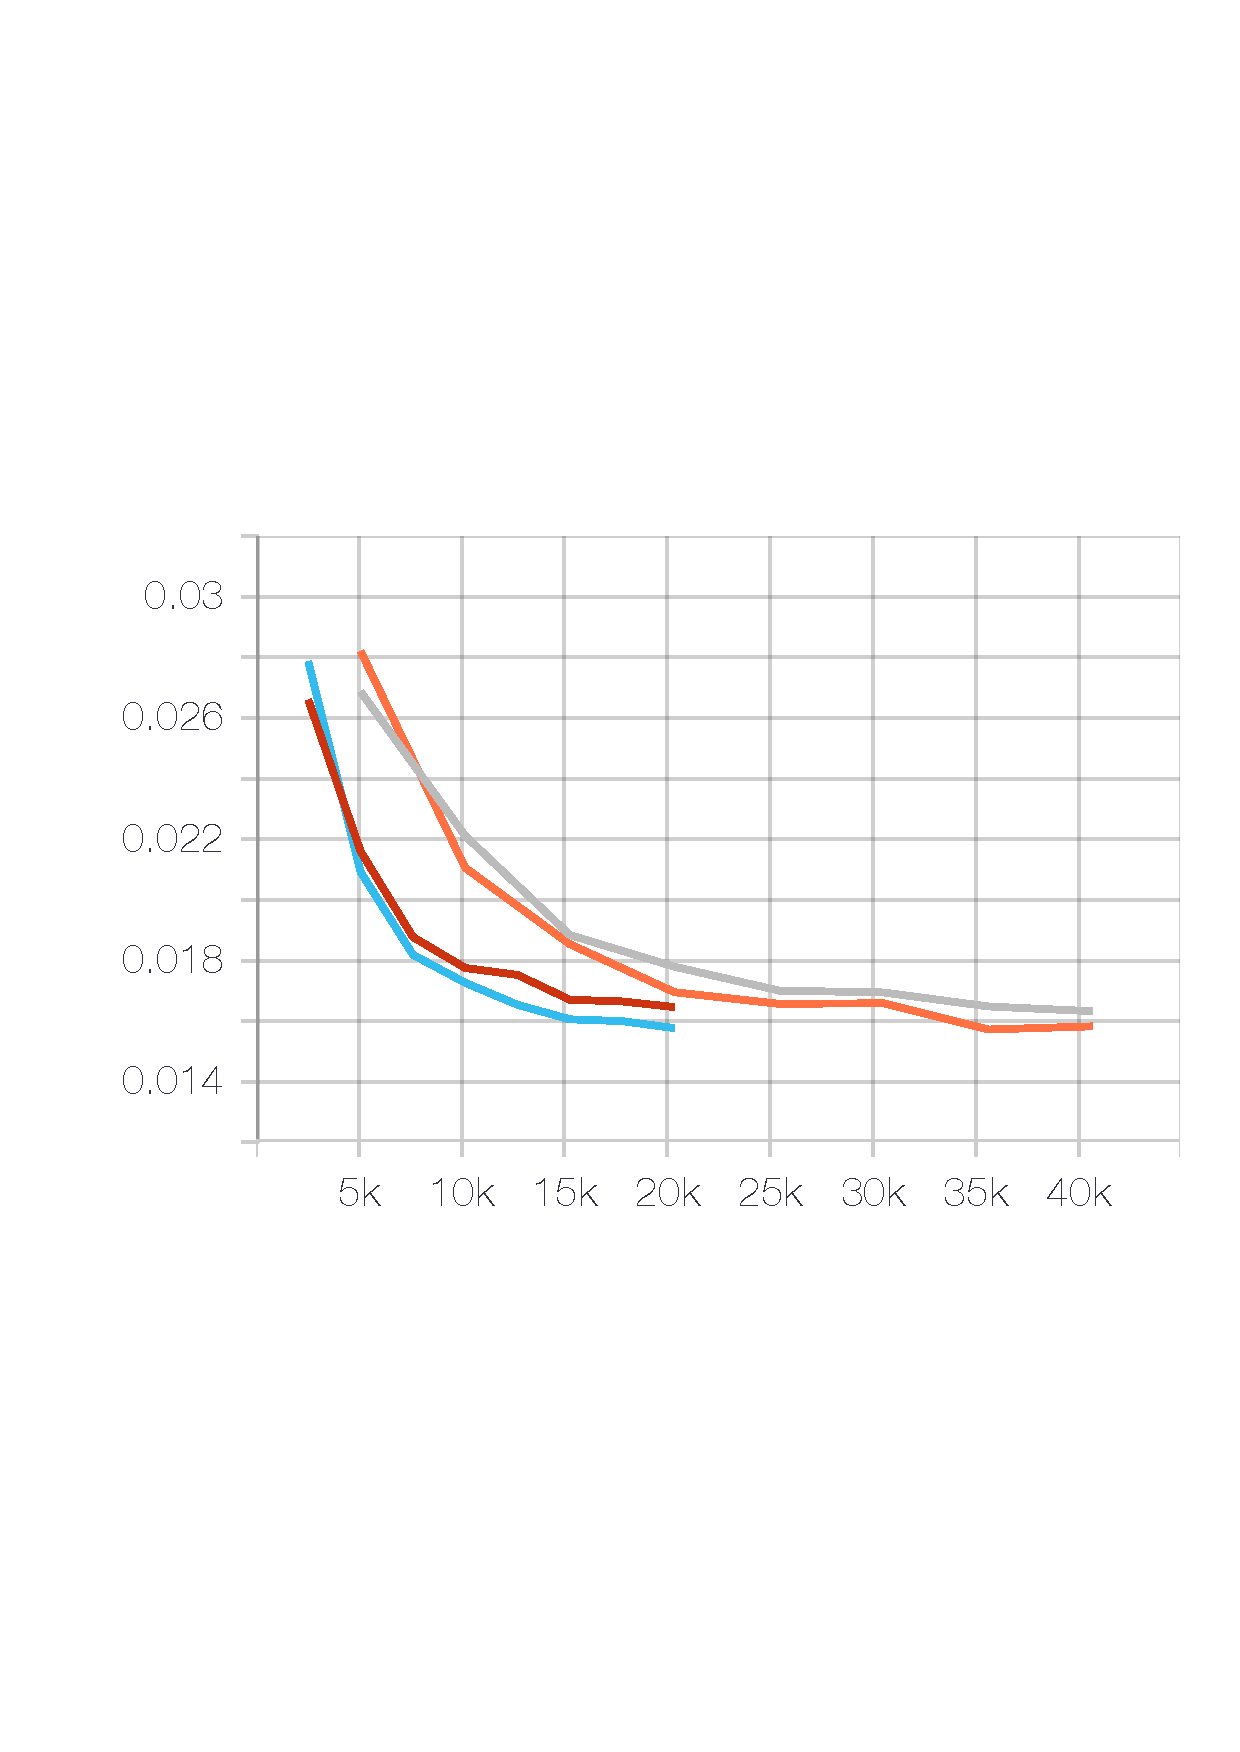
\includegraphics[width=\linewidth]{figures/grid_model_1}
	\captionof{figure}{Validation losses for model 1  (\textit{blue}: [bs=64, nf=64], \textit{red}: [bs=64, nf=32], \textit{orange}: [bs=32, nf=64], \textit{grey}: [bs=32, nf=32])}
	\label{fig:val_grid}
\end{Figure}

From the visual results in figures \ref{fig:imgs_bs32_nf32}, \ref{fig:imgs_bs32_nf64}, 
	\ref{fig:imgs_bs64_nf32} and \ref{fig:imgs_bs64_nf64} it is also becomes clear that higher batch sizes and more feature maps improve the reconstructed image. The images suggest that higher batch sizes cause the model to generalize better, since more faces are seen before the model's weights are updated. Intuitively, a deeper model with more feature maps can encode finer detail, hence increasing photorealism. 
	
\textbf{Experiment 3}: Motivated by this we trained more models with a higher number of feature maps $n_f$ and higher batch sizes. We train these networks with 10 maximum epochs. In figure \ref{fig:val_grid_2} we compare two deeper models with the previously best performing baseline model [bs=64, nf=64] and notice that increasing batch size and network depth even more does not yield lower loss values. As expected the quality of the visual results in figures \ref{fig:imgs_bs128_nf128} and \ref{fig:imgs_bs256_nf128} are at most comparable with our baseline model in figure \ref{fig:imgs_bs64_nf64} but certainly do not outperform it.

\begin{Figure}
	\centering 
	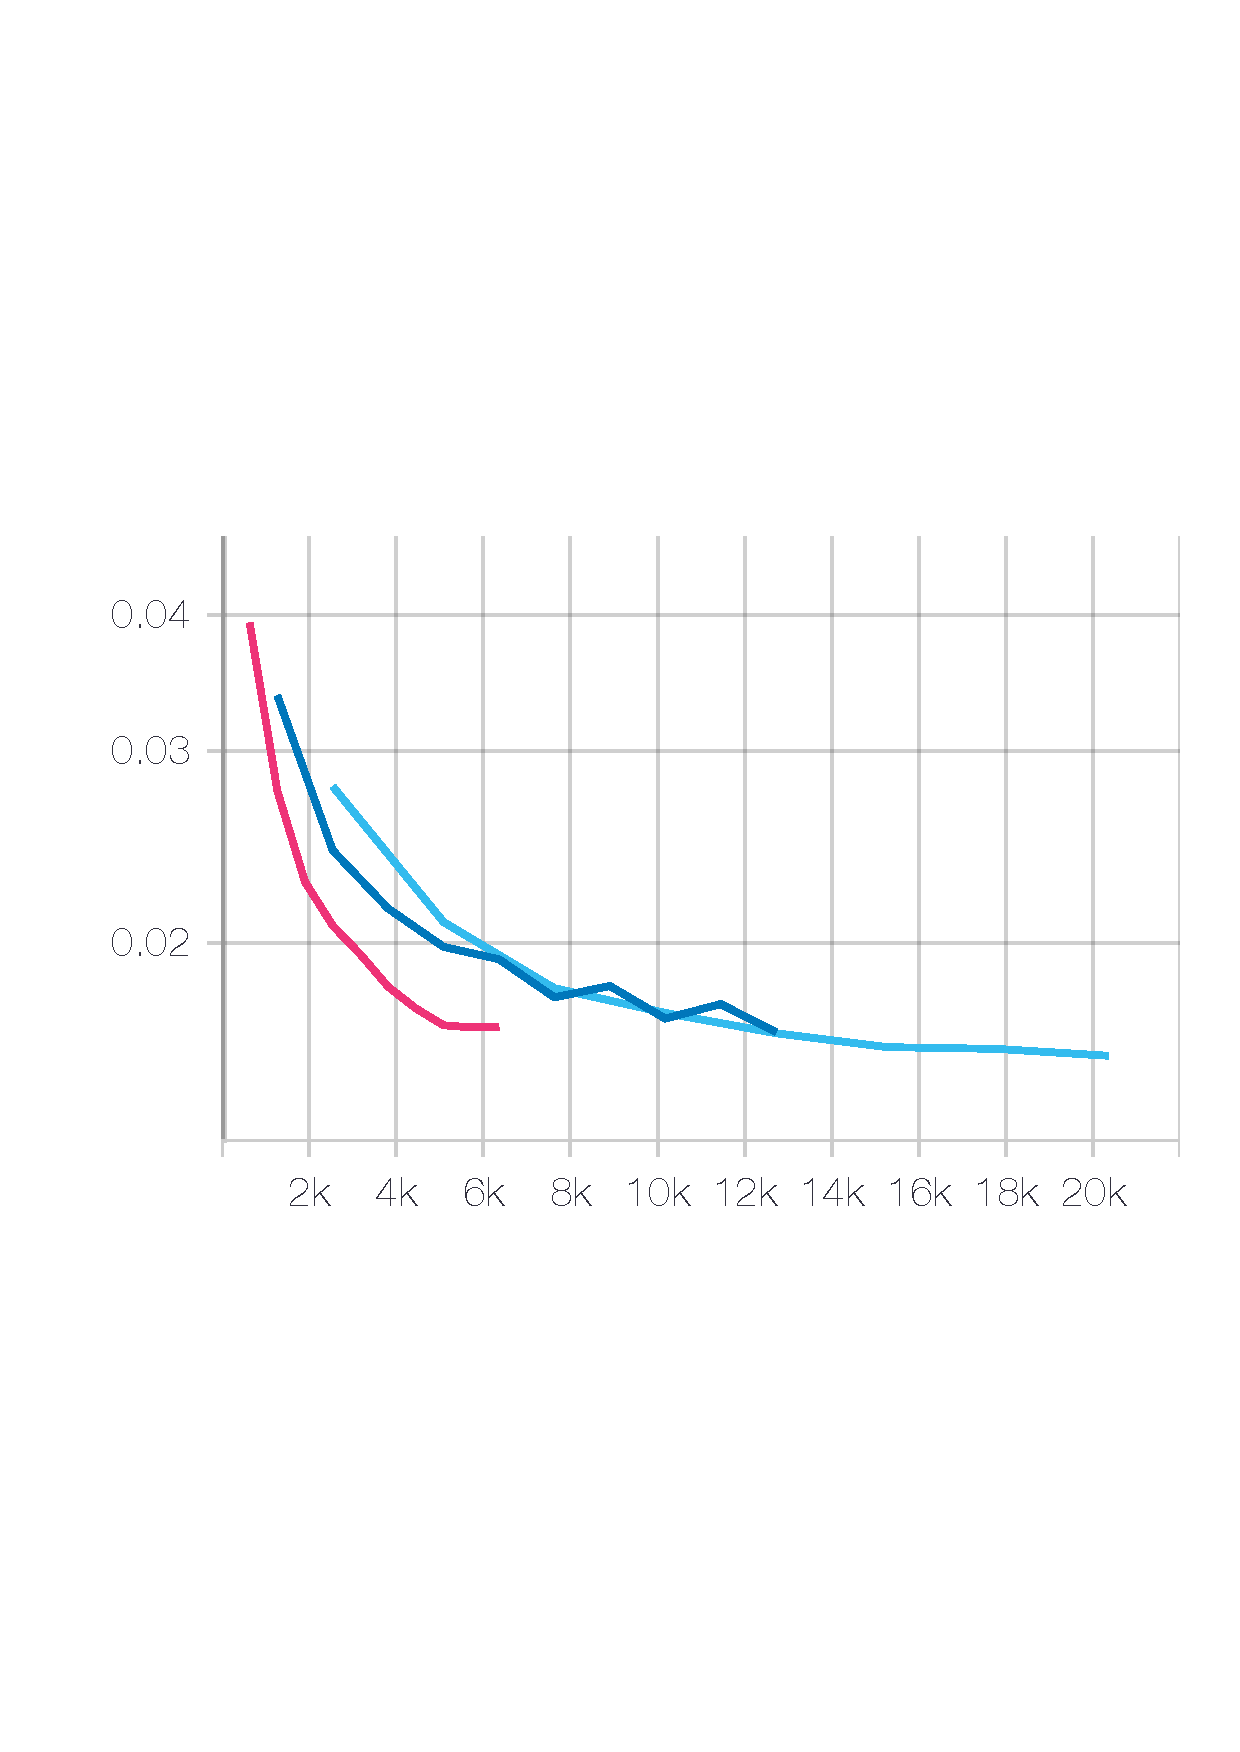
\includegraphics[width=\linewidth]{figures/avg_val_loss_2}
	\captionof{figure}{Validation losses for model 1  (\textit{light blue}: [bs=64, nf=64], \textit{dark blue}: [bs=128, nf=128], \textit{pink}: [bs=256, nf=128])}
	\label{fig:val_grid_2}
\end{Figure}

\printbibliography

\end{multicols}


\begin{figure}[p]	
	\vspace{1cm}
	\centering 
	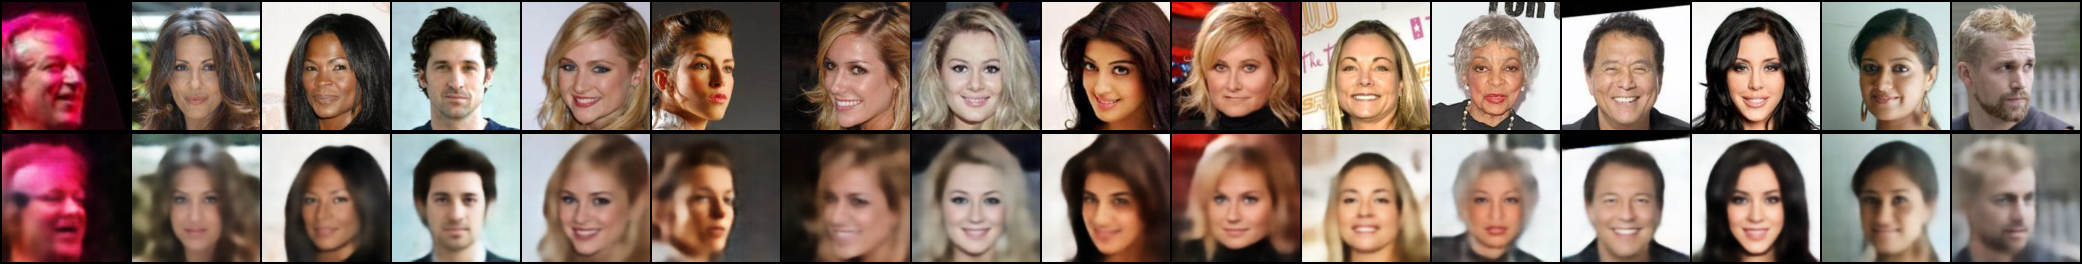
\includegraphics[width=0.95\linewidth]{figures/bs32_nf32}
	\caption{Test images produced by model 1 with [bs=32, nf=32]}
	\label{fig:imgs_bs32_nf32}
\end{figure}
\begin{figure}[p]
	\centering 
	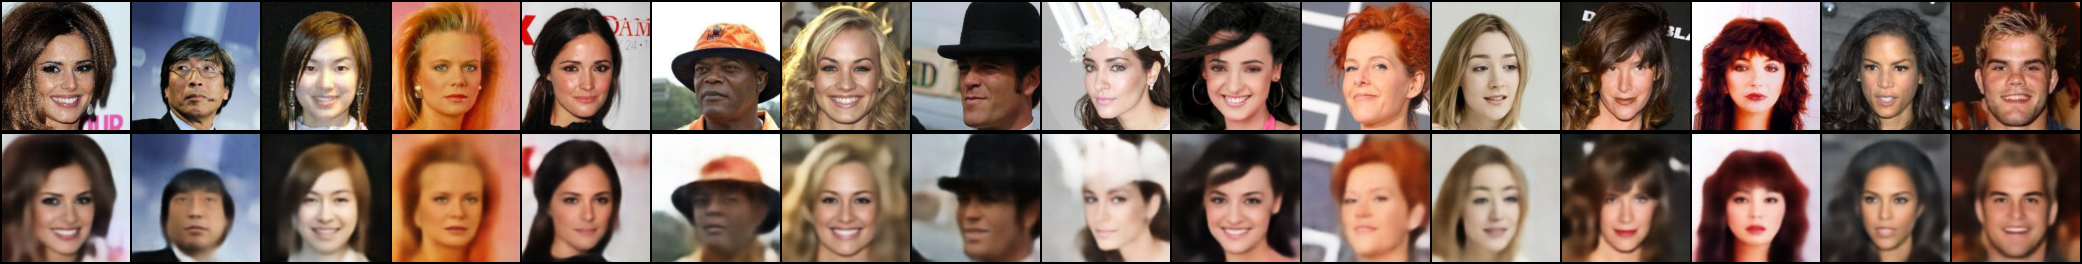
\includegraphics[width=0.95\linewidth]{figures/bs32_nf64}
	\caption{Test images produced by model 1 with [bs=32, nf=64]}
	\label{fig:imgs_bs32_nf64}
\end{figure}
\begin{figure}[p]
	\centering 
	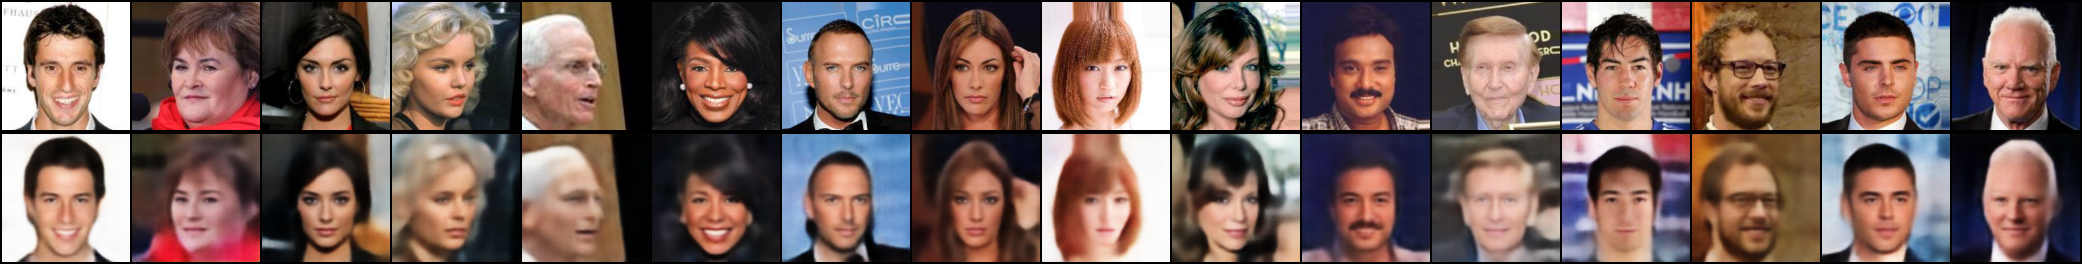
\includegraphics[width=0.95\linewidth]{figures/bs64_nf32}
	\caption{Test images produced by model 1 with [bs=64, nf=32]}
	\label{fig:imgs_bs64_nf32}
\end{figure}
\begin{figure}[p]
	\centering 
	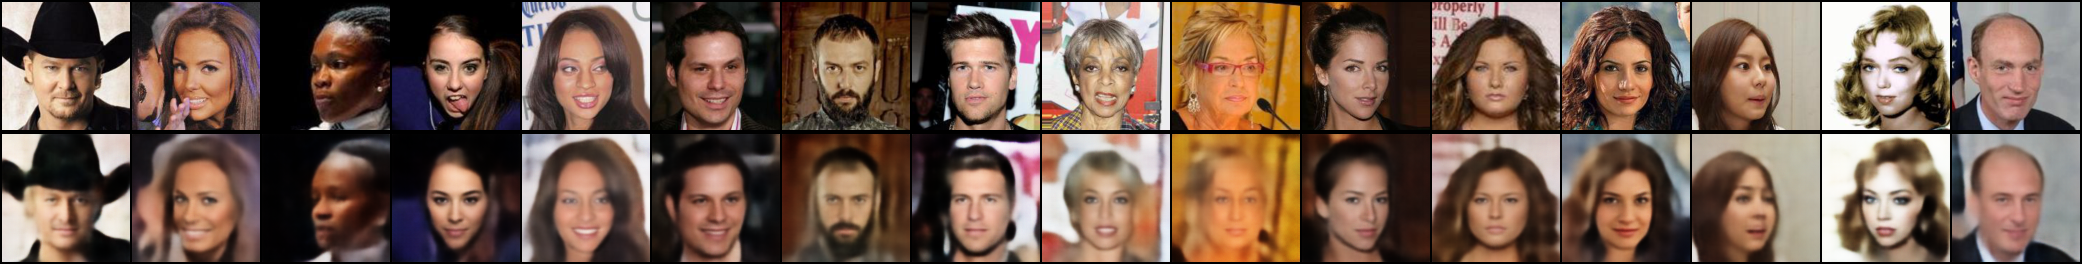
\includegraphics[width=0.95\linewidth]{figures/bs64_nf64}
	\caption{Test images produced by model 1 with [bs=64, nf=64]}
	\label{fig:imgs_bs64_nf64}
\end{figure}
\begin{figure}[p]
	\centering 
	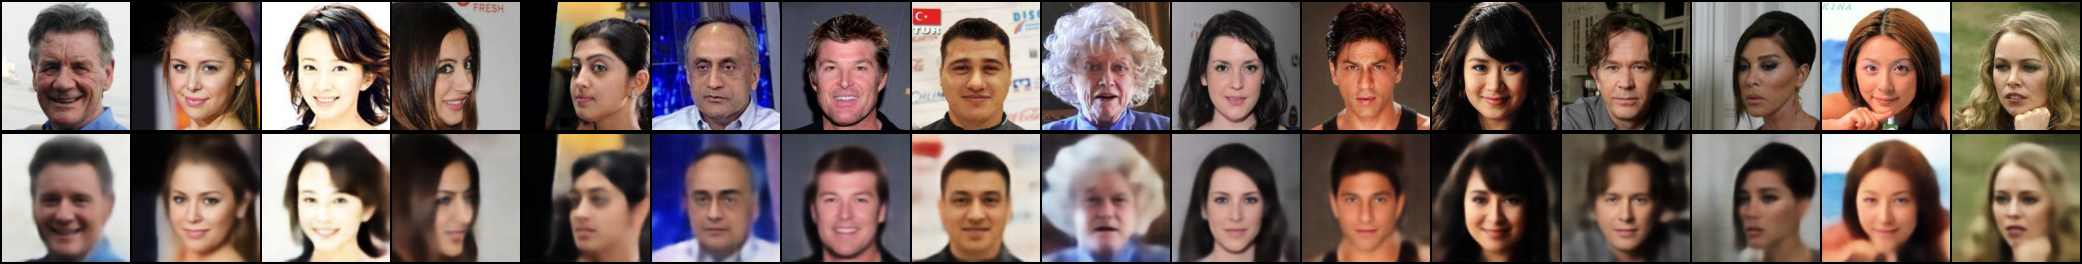
\includegraphics[width=0.95\linewidth]{figures/bs128_nf128}
	\caption{Test images produced by model 1 with [bs=128, nf=128]}
	\label{fig:imgs_bs128_nf128}
\end{figure}
\begin{figure}[p]
	\centering 
	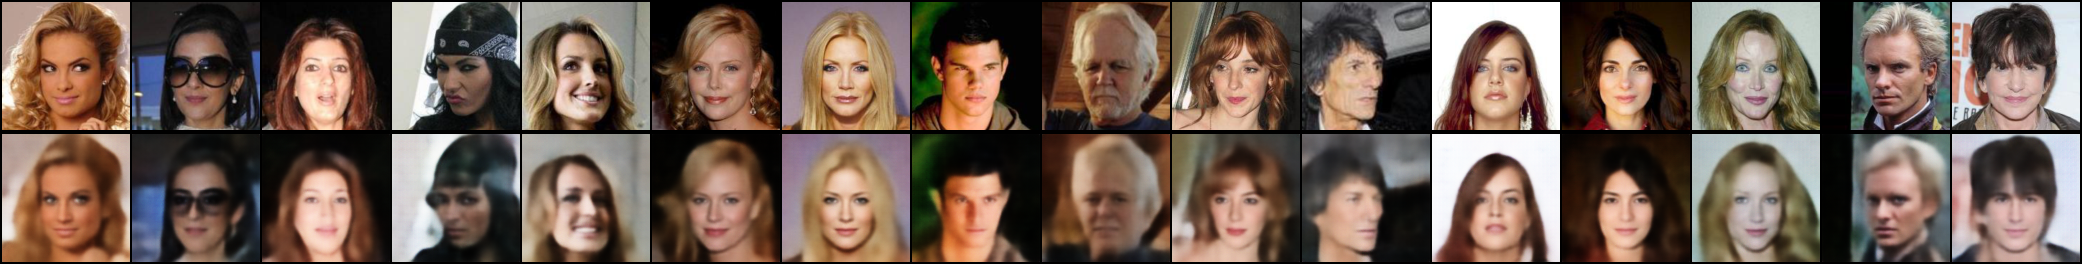
\includegraphics[width=0.95\linewidth]{figures/bs256_nf128}
	\caption{Test images produced by model 1 with [bs=256, nf=128]}
	\label{fig:imgs_bs256_nf128}
\end{figure}


\end{document}